\documentclass[first=dgreen,second=purple,presentation]{elecslides}
%\documentclass{elecslides} % DEFAULT
%\documentclass[first=purple,second=lgreen,logo=redque,normaltitle,nofoot]{aaltoslides} % SOME OPTION EXAMPLES

\usepackage[latin9]{inputenc}
\usepackage[T1]{fontenc}
\usepackage{graphicx}
\usepackage{amssymb,amsmath}
\usepackage{url}
\usepackage{animate}
\usepackage{media9}
\usepackage{tabularx}
\usepackage{colortbl}

\usepackage{lcg}
\reinitrand[first=1, last=3, seed=-1]
\newcommand{\alogoname}[1]{Aalto_ELEC_EN_13_RGB_#1.png}

\rand
%\renewcommand{\smalllogo}{\includegraphics[height=\smalllogoheight]{\alogoname{\arabic{rand}}}}
\renewcommand{\smalllogo}{\includegraphics[height=\smalllogoheight]{\alogoname{1}}}

\graphicspath{{.}{../pics/}}


\mode<presentation>
{
  \setbeamercovered{transparent}
}

\mode<handout>
{
  %\beamertemplatesolidbackgroundcolor{black!5}
}

\title{Stochastic (Partial) Differential Equations and Gaussian Processes}

\aaltofootertext{S(P)DEs and GPs}{Simo S\"arkk\"a}{\insertframenumber\,/\,\inserttotalframenumber\ }

\author{{\bf Simo S\"arkk\"a}}

\institute{Aalto University, Finland}

\date{}

%\date{Version 1.0, \today}

\AtBeginSection[]
{
  \begin{frame}<beamer>
    \frametitle{Contents}
    \tableofcontents[currentsection]
  \end{frame}
}
\begin{document}

%%%%%%%%%%%%%%%%%%%%%%%%%%%%%%%%%%%%%%%%%%%%%%%%%%%%%%%%%%%%%%%%%%%%%%%%%%%%%%%%%%%%%%%%%%%%%

\aaltotitleframe

\begin{frame}
  \frametitle{Contents}
  \tableofcontents[pausesections]
  % You might wish to add the option [pausesections]
\end{frame}

%%%%%%%%%%%%%%%%%%%%%%%%%%%%%%%%%%%%%%%%%%%%%%%%%%%%%%%%%%%%%%%%%%%%%%%%%%%%%%%%%%%%%%%%%%%%%

\section{Motivating applications}

\begin{frame}
 \frametitle{Magneto- and Electroencephalography (MEG \& EEG)}

\begin{itemize}[<+->]
\item \alert{Unknown}: Time course of amplitudes of dipole sources.
 \item \alert{Observed}: Electromagnetic field (potential / flux).  
 \end{itemize}
 \begin{center}
 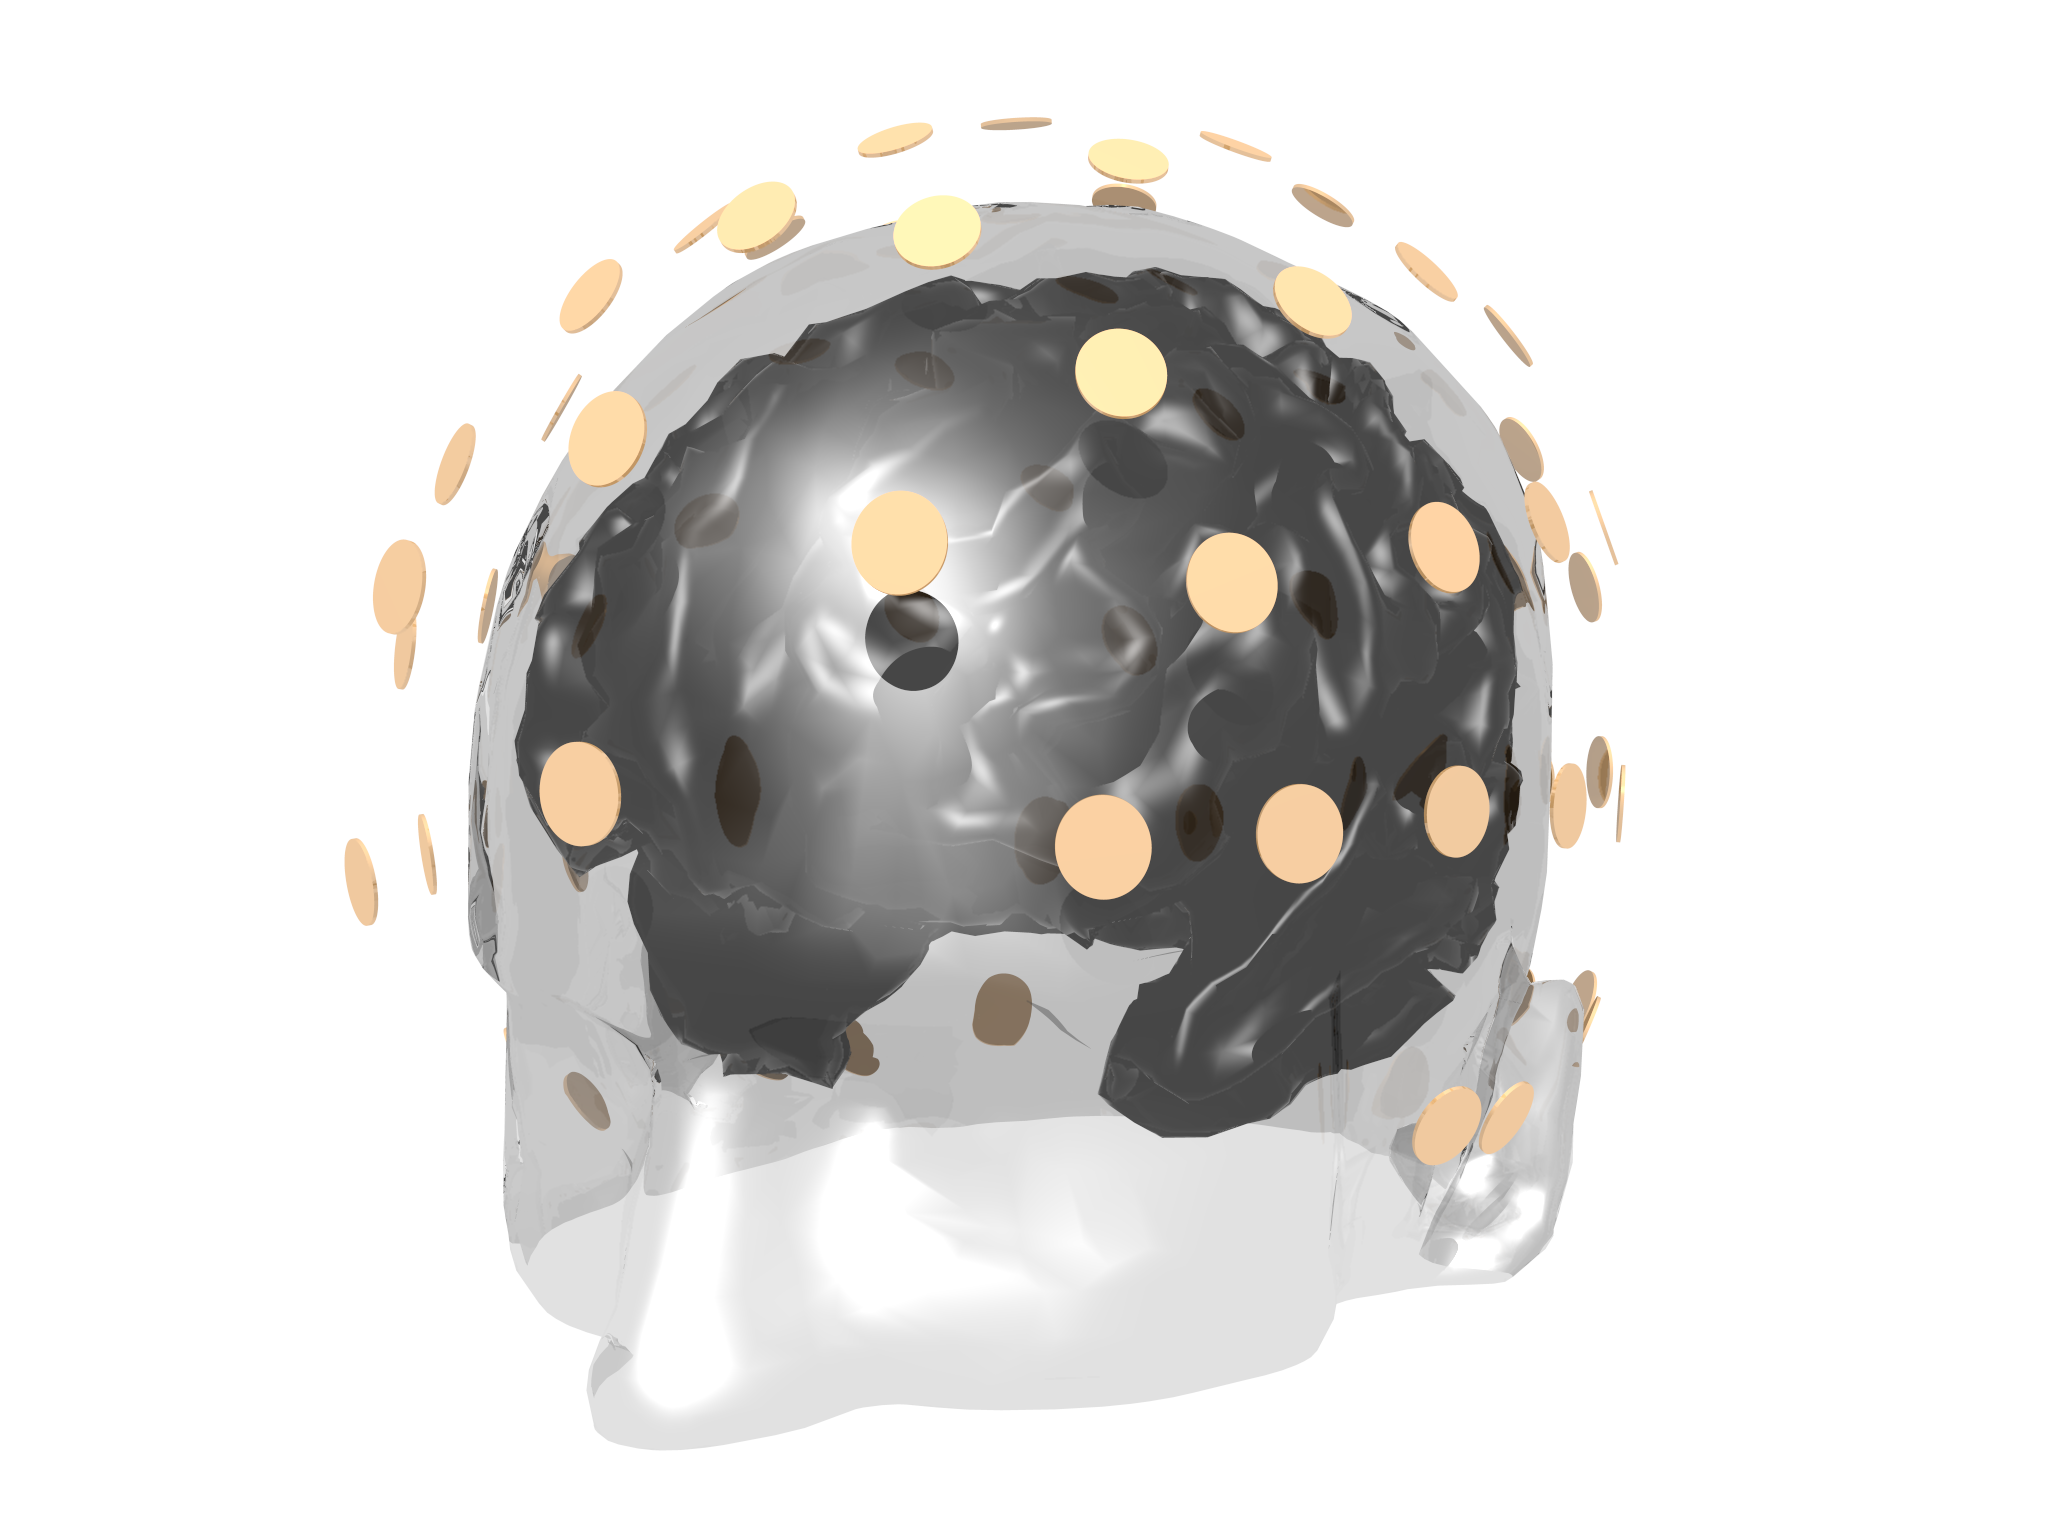
\includegraphics[width=0.6\textwidth]{head-col}
 \end{center}
\end{frame}

\begin{frame}
 \frametitle{Electrical Impedance and Capacitance Tomography (EIT \& ECT)}

 \begin{itemize}[<+->]
 \item \alert{Unknown}: Conductivity/permittivity constants.
 \item \alert{Observed}: Impedances on boundary.  
 \end{itemize}
 \begin{center}
 \includegraphics[width=0.6\textwidth]{rocsole}
  
 {\tiny Source: Rocsole Ltd. -- www.rocsole.com}
 \end{center}
\end{frame}

\begin{frame}
 \frametitle{Magnetic field mapping}

\begin{itemize}[<+->]
\item \alert{Unknown}: Magnetic field (or actually the corresponding potential).
\item \alert{Observed}: Point measurements of the magnetic field.  
\end{itemize}
\begin{center}
\includegraphics[width=0.4\textwidth]{table-surf}
  
\end{center}
\end{frame}

\begin{frame}
 \frametitle{Machine learning and Kriging}

 \begin{itemize}[<+->]
 \item \alert{Unknown}: Class labels or missing spatial values.
 \item \alert{Observed}: Subset (training set) of class labels, spatial values, and predictors. 
 \end{itemize}
 \begin{center}
 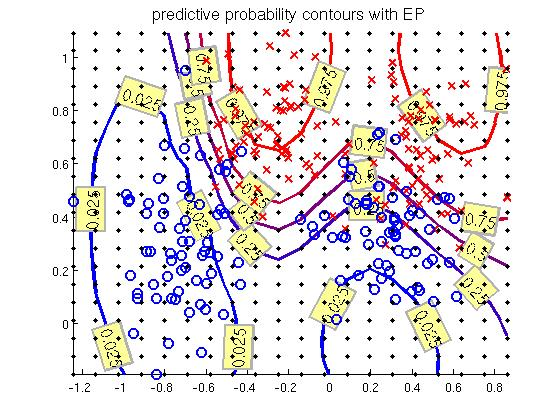
\includegraphics[width=0.57\textwidth]{demo_classific2}
 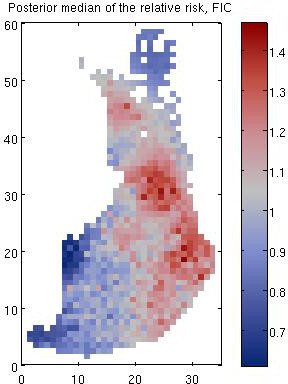
\includegraphics[width=0.3\textwidth]{spatial1_pic1}
 \end{center}
\end{frame}

\begin{frame}
 \frametitle{Target Tracking and Location Sensing}

 \begin{itemize}[<+->]
 \item \alert{Unknown}: Target trajectories and velocities.
 \item \alert{Observed}: Direction or inertial measurements.  
 \end{itemize}
 \begin{center}
 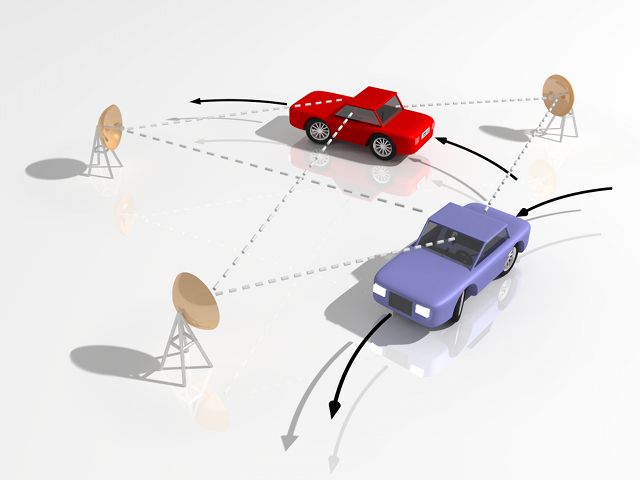
\includegraphics[width=0.6\textwidth]{tracking2-col}
 \end{center}
\end{frame}

%%%%%%%%%%%%%%%%%%%%%%%%%%%%%%%%%%%%%%%%%%%%%%%%%%%%%%%%%%%%%%%%%%%%%%%%%%%%%%%%%%%%%%%%%%%%%

\section{Using SPDE solvers on Gaussian processes}

\begin{frame}{Gaussian process regression models and inverse problems}

 \begin{itemize}[<+->]
 \item A typical \alert{statistical inverse problem}:
\begin{equation}
\begin{split}
  f(\mathbf{x}) &\sim \mathrm{GP}(m(\mathbf{x}),k(\mathbf{x},\mathbf{x}')) \\
  \mathbf{y} &= \boldsymbol{\mathcal{H}} \, f(\mathbf{x}) + \boldsymbol{\varepsilon} %, \qquad \varepsilon \sim \mathrm{N}(\mathbf{0},\Sigma),
\end{split}
\nonumber
\end{equation}

\item The \alert{operator matrix} $\boldsymbol{\mathcal{H}}$ encodes \alert{physics} into the model.

\item The \alert{mean} $m(\mathbf{x})$ and \alert{covariance function} $k(\mathbf{x},\mathbf{x}')$ encode the prior information on $f(\mathbf{x})$.

\item In plain \alert{Gaussian process regression} we have
\begin{equation}
\begin{split}
\boldsymbol{\mathcal{H}} \, f(\mathbf{x}) = \begin{pmatrix}
  f(\mathbf{x}_1) \\ \vdots \\ f(\mathbf{x}_n))
  \end{pmatrix}
\end{split}
\nonumber
\end{equation}

 \end{itemize}

\end{frame}


\begin{frame}{Gaussian process regression models and inverse problems (cont.)}

 \begin{itemize}[<+->]
 \item \alert{Temporal} models (models with single input):
\begin{equation}
\begin{split}
  f(t) &\sim \mathrm{GP}(m(t),k(t,t')) \\
  \mathbf{y} &= \boldsymbol{\mathcal{H}} \, f(t) + \boldsymbol{\varepsilon} %, \qquad \varepsilon \sim \mathrm{N}(\mathbf{0},\Sigma),
\end{split}
\nonumber
\end{equation}
 
\item \alert{Spatio-temporal} models:
\begin{equation}
\begin{split}
  f(\mathbf{x},t) &\sim \mathrm{GP}(m(\mathbf{x},t),k(\mathbf{x},t;\mathbf{x}',t')) \\
  \mathbf{y} &= \boldsymbol{\mathcal{H}} \, f(\mathbf{x},t) + \boldsymbol{\varepsilon} %, \qquad \varepsilon \sim \mathrm{N}(\mathbf{0},\Sigma),
\end{split}
\nonumber
\end{equation}

\item All of these can be recasted as \alert{statistical estimation on a stochastic partial differential equation (SPDE) model}.

\end{itemize}
\end{frame}



\begin{frame}{Why use S(P)DE solvers for GPs?}

\begin{itemize}[<+->]
\item The $O(n^3)$ \alert{computational complexity} is always a challenge.
%\item E.g. \alert{Inducing point methods}, \alert{grid-FFT}, \alert{compact support} -- but we need more.
\item \alert{Latent force models} combine PDE/ODEs with GPs.
\item What do we get:
\begin{itemize}[<+->]
\item \alert{Sparse approximations} developed for SPDEs.
\item \alert{Reduced rank} Fourier/basis function approximations.
\item The use of \alert{Markov properties} and Markov approximations.
\item \alert{State-space} methods for SDEs/SPDEs.
\item Path to \alert{non-Gaussian processes}.
\end{itemize}
\item Downsides:
\begin{itemize}[<+->]
\item Approximations of non-parametric models with parametric models.
\item Approximations of a non-Markovian models as Markovian.
\item Mathematics can become messy.
\end{itemize}
\end{itemize}
\end{frame}

\begin{frame}{Kernel vs. SPDE representations of GPs}

\begin{tabularx}{0.98\textwidth}{ | p{0.38\textwidth} | p{0.52\textwidth} | }
\hline
\cellcolor{blue!25}GP model $\mathbf{x} \in \mathbb{R}^d, t \in \mathbb{R}$ & \cellcolor{blue!25}Equivalent Static SPDE model \\
\hline
\hline
Homogenous $k(\mathbf{x},\mathbf{x}')$ &
SPDE model
\begin{equation}
  \mathcal{L} \, f(\mathbf{x}) = w(\mathbf{x})
\nonumber
\end{equation}
%translation invariant operator $\mathcal{L}$
\\
\hline
Stationary $k(t,t')$ &
State-space/It\^o-SDE model 
\begin{equation}
%\frac{d\mathbf{f}(t)}{dt} = \mathbf{A} \, \mathbf{f}(t) + \mathbf{L} \, w(t)
d\mathbf{f}(t) = \mathbf{A} \, \mathbf{f}(t) \, dt + \mathbf{L} \, dW(t)
\nonumber
\end{equation}
\\
\hline
Homogenous/stationary $k(\mathbf{x},t;\mathbf{x}',t')$ & 
Stochastic evolution equation
\begin{equation}
\partial_t \mathbf{f}(\mathbf{x},t)
= \mathcal{A}_x \, \mathbf{f}(\mathbf{x},t) \, dt + \mathbf{L} \, dW(\mathbf{x},t)
%, \quad
%f = \mathbf{C} \, \mathbf{f}
\nonumber
\end{equation}
\\
\hline
\end{tabularx}

\end{frame}

%%%%%%%%%%%%%%%%%%%%%%%%%%%%%%%%%%%%%%%%%%%%%%%%%%%%%%%%%%%%%%%%%%%%%%%%%%%%%%%%%%%%%%%%%%%%%


\section{What do the SPDE methods then look like?}

\begin{frame}{Basic idea of SPDE inference on GPs [1/2]}

\begin{itemize}[<+->]
\item Consider e.g. the \alert{stochastic partial differential equation}:
\begin{equation}
  \frac{\partial^2 f(x,y)}{\partial x^2}
  + \frac{\partial^2 f(x,y)}{\partial y^2} -\lambda^2 \, f(x,y)
  = w(x,y)
%\label{eq:whittle}
\nonumber
\end{equation}

\item Fourier transforming gives the \alert{spectral density}:
%
\begin{equation}
  S(\omega_x,\omega_y)  \propto 
     \left( \lambda^2 + \omega_x^2 + \omega_y^2 \right)^{-2}. 
\nonumber
\end{equation}
%
\item Inverse Fourier transform gives the \alert{covariance function}:
{\small
\begin{equation}
  k(x,y;x',y')
  = \frac{\sqrt{(x-x')^2 + (y-y')^2}}{2\lambda} \, 
  K_1(\lambda \, \sqrt{(x-x')^2 + (y-y')^2})
\nonumber
\end{equation}
}

\item But this is just the \alert{Mat\'ern covariance function}.

\item The corresponding \alert{RKHS} is a \alert{Sobolev space}.

%\item Any probabilistic (weak) \alert{question on GP} with covariance $k$ is equivalent to the \alert{question on the SPDE model}.
\end{itemize}

\end{frame}


\begin{frame}{Basic idea of SPDE inference on GPs [2/2]}
\begin{itemize}[<+->]
\item More generally, \alert{SPDE} for some linear operator $\mathcal{L}$:
\begin{equation}
  \mathcal{L} \, f(\mathbf{x}) = w(\mathbf{x})
\nonumber
\end{equation}

\item Now $f$ is a GP with \alert{precision and covariance operators}:
\begin{equation}
\begin{split}
  \mathcal{K}^{-1} &= \mathcal{L}^* \, \mathcal{L} \\
  \mathcal{K} &= (\mathcal{L}^* \, \mathcal{L})^{-1}
\end{split}
\nonumber
\end{equation}

\item \alert{Idea:} approximate $\mathcal{L}$ or $\mathcal{L}^{-1}$ using PDE/ODE methods:
\begin{enumerate}[<+->]
\item \alert{Finite-differences/FEM} methods lead to \alert{sparse precision approximations}.
\item \alert{Fourier/basis-function} methods lead to \alert{reduced rank covariance approximations}.
\item \alert{Spectral factorization} leads to state-space (Kalman) methods which are \alert{time-recursive} (or sparse in precision).
\end{enumerate}

%\item In particular, when $\mathbf{x} \in \mathbb{R}$, we can use \alert{Kalman filtering} which scales as $O(n)$.
\end{itemize}

\end{frame}

\begin{frame}{Finite-differences/FEM -- sparse precision}

\begin{block}{}
\begin{columns}
\begin{column}{0.55\textwidth}
\begin{itemize}[<+->]
\item Basic idea:
{\small
\begin{equation}
\begin{split}
  \frac{\partial f(x)}{\partial x} & \approx \frac{f(x + h) - f(x)}{h} \\
  \frac{\partial^2 f(x)}{\partial x^2} & \approx \frac{f(x + h) - 2 f(x) + f(x - h)}{h^2} \\
\end{split}
\nonumber
\end{equation}
}
\end{itemize}
\end{column}
\begin{column}{0.45\textwidth}
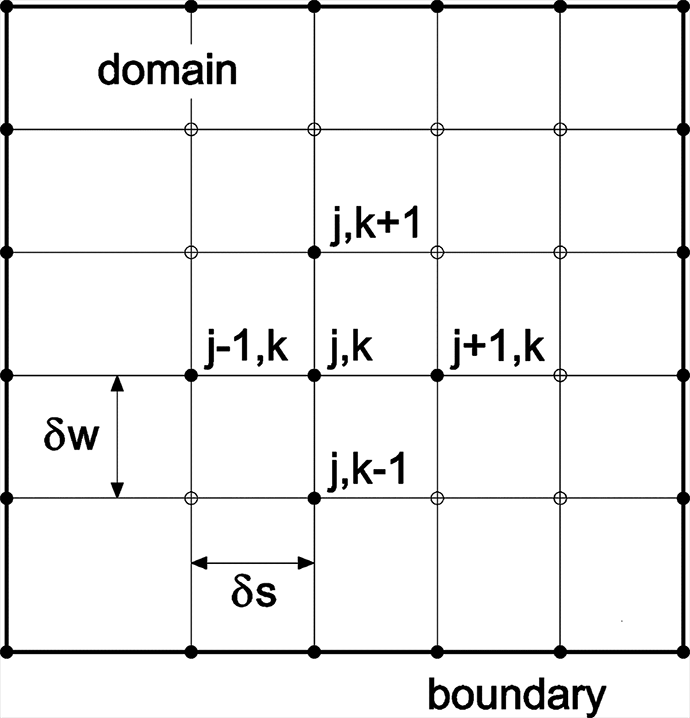
\includegraphics[width=0.45\columnwidth]{fd}
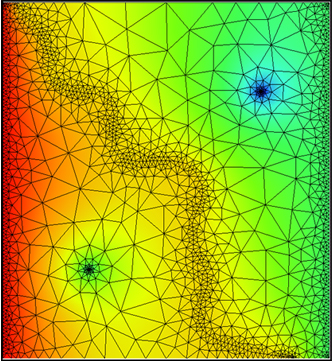
\includegraphics[width=0.45\columnwidth]{fem}
\end{column}
\end{columns}
\end{block}

\begin{itemize}[<+->]
\setcounter{enumi}{2}
\item We get an SPDE approximation $\mathcal{L} \approx \mathbf{L}$, where $\mathbf{L}$ is \alert{sparse} %e.g. [Lindgren et al. 2011, Roininen \ldots S\"arkk\"a 2016].
\item The \alert{precision operator} approximation is then \alert{sparse}:
\begin{equation}
\begin{split}
  \mathcal{K}^{-1} \approx \mathbf{L}^\mathsf{T} \, \mathbf{L} = \text{sparse}\\
\end{split}
\nonumber
\end{equation}

\item $\mathcal{L}$ need to be approximated as \alert{integro-differential operator}.

\item Requires formation of a \alert{grid}, but parallelizes well.

\end{itemize}


\end{frame}

%[XX,YY] = meshgrid(0:0.01:1,0:0.01:1);
%clf;
%for i=1:3
%    for j=1:3
%        subplot(3,3,j+3*(i-1));
%        pcolor(XX,YY,sin(2*pi*i*XX) .* sin(2*pi*j*YY));
%        axis off;
%        shading flat
%    end
%end
%print -dpng fourier.png;
%


\begin{frame}{Classical and random Fourier methods -- reduced rank approximations and FFT}
\begin{block}{}
\begin{columns}
\begin{column}{0.5\textwidth}
\begin{itemize}[<+->]
\item Approximation:
{\small
\begin{equation}
\begin{split}
  f(\mathbf{x}) &\approx \sum_{\mathbf{k} \in \mathbb{N}^d}
    c_\mathbf{k} \, \exp\left(2 \pi \, \mathrm{i} \, \mathbf{k}^\mathsf{T} \, \mathbf{x} \right) \\
    c_\mathbf{k} &\sim \text{Gaussian}
\end{split}
\nonumber
\end{equation}
}
\end{itemize}
\end{column}
\begin{column}{0.4\textwidth}
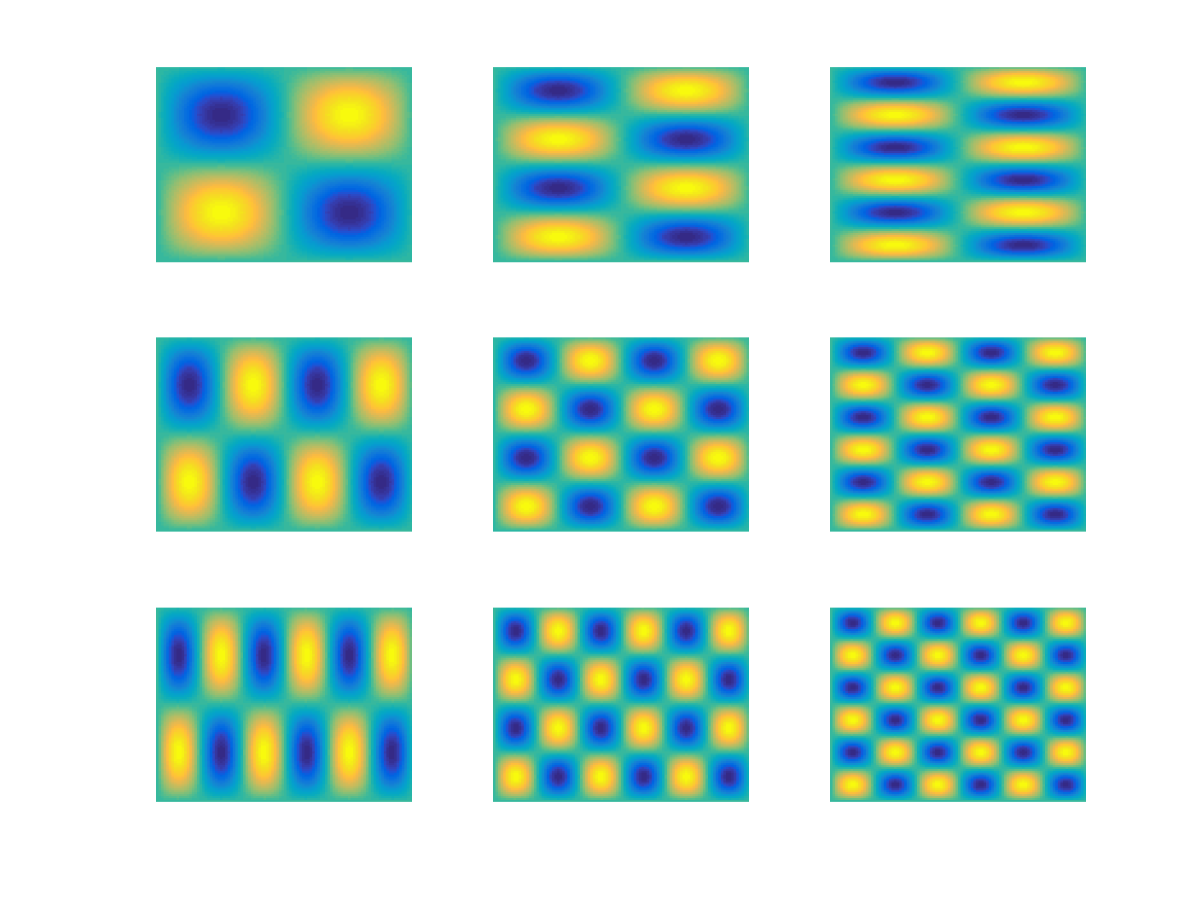
\includegraphics[width=1.0\columnwidth]{fourier}
\end{column}
\end{columns}
\end{block}

\begin{itemize}[<+->]
\setcounter{enumi}{2}
\item We use \alert{less coefficients} $c_\mathbf{k}$ than the \alert{number of data points}.
\item Leads to \alert{reduced-rank covariance approximations}
\begin{equation}
\begin{split}
  k(\mathbf{x},\mathbf{x}') \approx \sum_{|\mathbf{k}| \le N} 
    \sigma^2_{\mathbf{k}} \, \exp\left(2 \pi \, \mathrm{i} \, \mathbf{k}^\mathsf{T} \, \mathbf{x} \right)
    \, \exp\left(2 \pi \, \mathrm{i} \, \mathbf{k}^\mathsf{T} \, \mathbf{x}' \right)^*
\end{split}
\nonumber
\end{equation}
\item Truncated series, random frequencies, FFT, \ldots
\end{itemize}

\end{frame}

\begin{frame}{Hilbert-space/Galerkin methods -- reduced rank approximations}

\begin{block}{}
\begin{columns}
\begin{column}{0.5\textwidth}
\begin{itemize}[<+->]
\item Approximation:
{\small
\begin{equation}
\begin{split}
  f(\mathbf{x}) &\approx \sum_{i}
    c_i \, \phi_i(\mathbf{x}) \\
%    c_i &\sim \text{Gaussian} \\
    \langle \phi_i, \phi_j \rangle_H &\approx \delta_{ij},  \text{ e.g. } \nabla^2 \phi_i = -\lambda_i \, \phi_i
\end{split}
\nonumber
\end{equation}
}
\end{itemize}
\end{column}
\begin{column}{0.4\textwidth}
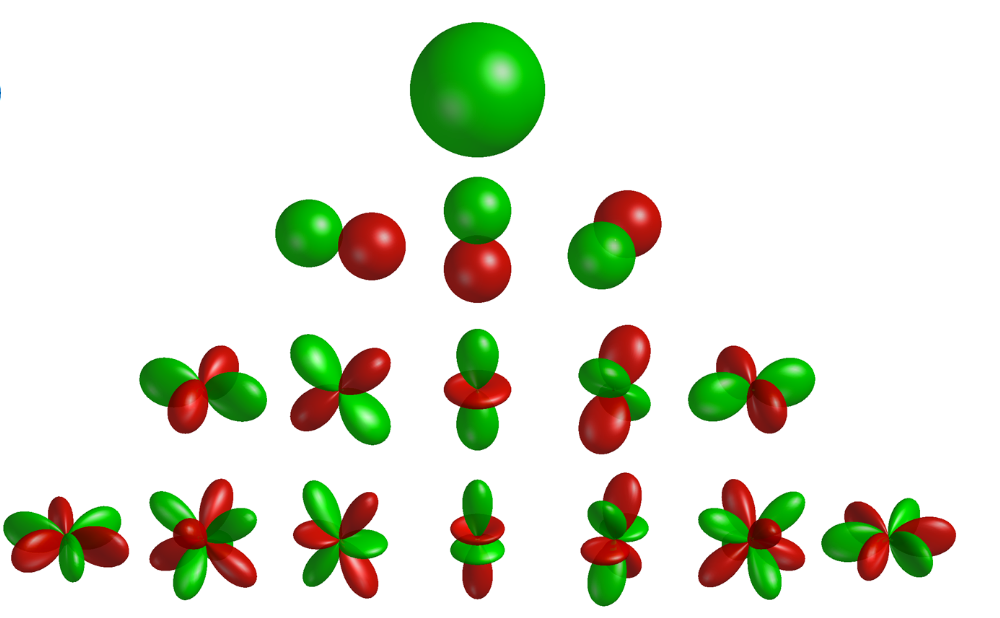
\includegraphics[width=1.0\columnwidth]{spherical}
\end{column}
\end{columns}
\end{block}

\begin{itemize}[<+->]
\setcounter{enumi}{2}
\item Again, use \alert{less coefficients} than the \alert{number of data points}.
\item \alert{Reduced-rank covariance approximations} such as
\begin{equation}
\begin{split}
  k(\mathbf{x},\mathbf{x}') \approx \sum_{i=1}^N  
    \sigma^2_i \, \phi_i(\mathbf{x}) \, \phi_i(\mathbf{x}').
\end{split}
\nonumber
\end{equation}
\item Wavelets, Galerkin, finite elements, \ldots
\end{itemize}

\end{frame}

\begin{frame}{State-space methods -- Kalman filters and sparse precision}
\begin{block}{}
\begin{columns}
\begin{column}{0.5\textwidth}
\begin{itemize}[<+->]
\item Approximation:
{\small
\begin{equation}
  S(\omega) \approx \frac{b_0 + b_1 \, \omega^2 + \cdots + b_M \, \omega^{2M}}
  {a_0 + a_1 \, \omega^2 + \cdots + a_N \, \omega^{2N}}
\nonumber
\end{equation}
}
\end{itemize}
\end{column}
\begin{column}{0.4\textwidth}
%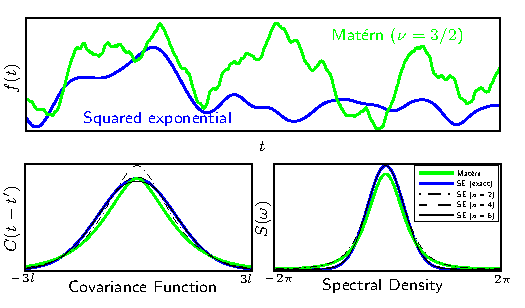
\includegraphics[width=0.7\columnwidth]{Sqexp-vs-Matern-1D}
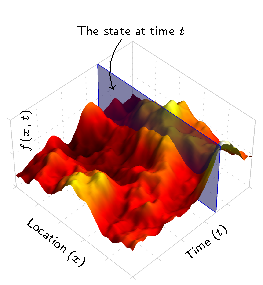
\includegraphics[width=0.6\columnwidth]{TikZ-temporal-figure}
\end{column}
\end{columns}
\end{block}
\begin{itemize}[<+->]
\setcounter{enumi}{2}
\item Results in a \alert{linear stochastic differential equation (SDE)}
\begin{equation}
%\frac{d\mathbf{f}(t)}{dt} = \mathbf{A} \, \mathbf{f}(t) + \mathbf{L} \, w(t)
d\mathbf{f}(t) = \mathbf{A} \, \mathbf{f}(t) \, dt + \mathbf{L} \, d\mathbf{W}
\nonumber
\end{equation}

\item More generally \alert{stochastic evolution equations}.

\item $O(n)$ GP regression with \alert{Kalman filters and smoothers}.

\item Parallel \alert{block-sparse precision} methods $\longrightarrow$ $O(\log n)$.
\end{itemize}
\end{frame}

\begin{frame}{State-space methods -- Kalman filters and sparse precision (cont.)}
  \begin{example}[Mat\'ern class 1d]
        The Mat\'ern class of covariance functions is
        %
\begin{equation*}
k(t,t') = \sigma^2 \,\frac{2^{1-\nu}}{\Gamma(\nu)}
\left(\frac{\sqrt{2\nu}}{\ell} |t-t'| \right)^{\nu} K_{\nu}
\left(\frac{\sqrt{2\nu}}{\ell}  |t-t'| \right).
\end{equation*}
        %
        When, e.g., $\nu = 3/2$, we have
\begin{equation*}
\begin{split}
d\mathbf{f}(t) &= 
\begin{pmatrix} 
0 & 1 \\
-\lambda^2 & -2\lambda
\end{pmatrix} \,\mathbf{f}(t) \, dt
+ 
\begin{pmatrix}
0\\
q^{1/2}
\end{pmatrix}\,dW(t), \\
f(t) &= \begin{pmatrix} 1 & 0 \end{pmatrix} \, \mathbf{f}(t).
\end{split}
\end{equation*} 
   \end{example}
\end{frame}

\begin{frame}{State-space methods -- Kalman filters and sparse precision (cont.)}
\begin{example}[2D Mat\'ern covariance function]
%
\begin{itemize}[<+->]
\item Consider a space-time Mat\'ern covariance function
%
  $$ k(x,t;x',t') = \sigma^2\frac{2^{1-\nu}}{\Gamma(\nu)}\left(\sqrt{2\nu}\,\frac{\rho}{
l}\right)^\nu K_\nu\left(\sqrt{2\nu}\,\frac{\rho}{l}\right). $$

where we have $\rho = \sqrt{(t-t')^2+ (x-x')^2}$, $\nu=1$ and $d=2$.

\item We get the following representation:
%
\begin{equation}
  d\mathbf{f}(x,t) = 
       \begin{pmatrix} 
        0 & 1 \\ 
%        \nabla^2-\lambda^2
%        & -2 \sqrt{\lambda^2-\nabla^2} 
        \frac{\partial^2}{\partial x^2} - \lambda^2
        & -2 \sqrt{\lambda^2 - \frac{\partial^2}{\partial x^2}}
      \end{pmatrix} \, \mathbf{f}(x,t) \, dt+ \begin{pmatrix} 0 \\ 1 \end{pmatrix} dW(x,t).
\nonumber
\end{equation}
%

%\item Example realization:
%
%  \begin{center}
%    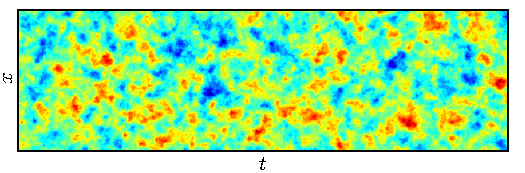
\includegraphics[width=6cm,keepaspectratio]{Matern-2D}
%  \end{center}%
%
\end{itemize}
\end{example}

\end{frame}

\section{Discussion and summary}

\begin{frame}{What then?}

\begin{itemize}[<+->]
\item We can \alert{exchange approximations} between the fields.
\item \alert{Inference} on the basis functions/point-locations/etc.
\item \alert{Non-Gaussian} processes, non-Gaussian likelihoods.
\item \alert{Hierarchical} (deep) \alert{SPDE models}.
\item \alert{Combined first-principles} and nonparametric models -- latent force models (LFM).
%\item \alert{Inverse problems} -- operators in measurement model.
\item \alert{State-space stochastic control} in Gaussian processes and LFMs.
%\item \alert{SPDE methods for SVMs}
%\item \alert{Kernel embedding of S(P)DEs}
\end{itemize}

\end{frame}

\begin{frame}{Summary}
\begin{itemize}[<+->]
\item Gaussian processes (GPs) can be used as \alert{priors in inverse problems}.
\item Applications in e.g. \alert{brain imaging, tomography, positioning, and Kriging}.
\item GPs have representations as \alert{solutions to SPDEs}.
\item SPDE methods can be used to \alert{speed up GP inference}.
\item In temporal models we can use \alert{Kalman/Bayesian filters and smoothers}.
\item Opens up new paths towards \alert{non-linear GP models}.
\end{itemize}
\end{frame}


%%%%%%%%%%%%%%%%%%%%%%%%%%%%%%%%%%%%%%%%%%%%%%%%%%%%%%%%%%%%%%%%%%%%%%%%%%%%%%%%%%%%%%%%%%%%%

\end{document}
